\chapter{Experiments and Results}
The main aim of this section is to assess the use of static features when involved in the characterisation of Android malware and benignware samples used to train detection tools. Thus, through
the use of several machine learning classifiers, it is studied if this combination with stacking methods is feasible and, if
so, to assess its performance when applied to build a machine learning aided Android malware
detection tools.

\section{1st Stage training experiments} \label{1ststagetrain}

For the 1st stage training step of our model, the selected ensemble classifiers were run with the Scikit-learn library for Python\cite{scikitlearn}.
They include AdaBoost, XGBoost, Catboost, Bagging Classifier, K-nearest neighbors, Neural network, Random Forest. 
All these ensemble classifiers were tested with the previously mentioned dataset through a 10-folds cross validation with accuracy scoring method showed below.

$$Accuracy = (TP+TN)/(TP+TN+FP+FN)$$
$$where: TP = \text{True positive}; FP = \text{False positive};$$$$TN = \text{True negative}; FN = \text{False negative}$$

For a better evaluation of the capacity of these algorithms to extract
and generalise conclusions, several experiments were conducted in order to judge the individual performance of the all models.
The results are shown in Table \ref{table:1ststage} and Figure \ref{fig:1ststage}

\begin{table}[htbp]
    \centering
    \caption{Experiments results on 1st training stage}
    \label{table:1ststage}
    \begin{adjustbox}{width=\textwidth}
        
    \begin{tabular}{|cccccccc|}
        \hline
        
        \textbf{Model} & \textbf{Activities CV} & \textbf{API calls CV} & \textbf{Opcodes CV} & \textbf{Permissions CV} & \textbf{Receivers CV} & \textbf{Services CV} & \textbf{System CV} \\ \hline
        LightGBM & 0.5094 & 0.8783 & 0.8519 & 0.7979 & 0.8486 & 0.5094 & 0.7866 \\ \hline
        Bagging & 0.5108 & \textbf{0.8817} & 0.8544 & 0.8094 & 0.8577 & 0.5099 & 0.7986 \\ \hline
        CatBoost & 0.5103 & 0.8762 & 0.8499 & 0.8048 & 0.8525 & 0.5031 & 0.7912 \\ \hline
        Neural Network & 0.5124 & 0.8518 & 0.8189 & 0.7841 & 0.8429 & 0.5092 & 0.7692 \\ \hline
        XGBoost & 0.5099 & 0.8740 & 0.8469 & 0.8008 & 0.8388 & 0.5094 & 0.7809 \\ \hline
        Random Forest & 0.5098 & 0.8238 & 0.8348 & 0.6143 & 0.7946 & 0.5064 & 0.7526 \\ \hline
        K-Neighbors & 0.5050 & 0.8466 & 0.8279 & 0.7817 & 0.8440 & 0.5116 & 0.7743 \\ \hline
        
        \end{tabular}

    \end{adjustbox}
    \end{table}

    \begin{figure}[htbp]
        \centering
        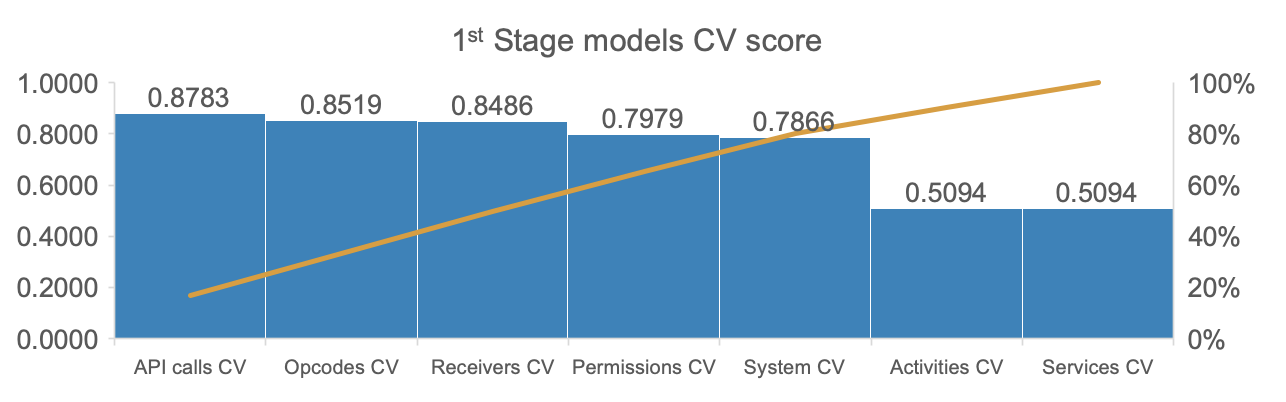
\includegraphics[width=\textwidth]{./Figure/1ststage.png}
        \caption{1st Stage models CV accuracy score average}
        \label{fig:1ststage}
      \end{figure}

 In particular, API
calls compose the most appropriate representation to build a machine learning classification
tool, exhibiting a 88.17\verb+%+ accuracy with a Bagging classifier. In general,
this algorithm obtains the best results overall.
% It is remarkable the fact that a combination of API calls with other also competitive features,
% such as opcodes or receivers, which have proved to be powerful at building detection mechanisms, does not lead to better values.

It is remarkable the fact that not only API calls has good results but also Opcodes and Receivers have proved to be powerful at building detection mechanisms as we can see in Figure \ref{fig:1ststage}. In contrast, we found that Activities and Services are to be less useful at building malware detection mechanisms.

\section{2nd Stage training experiments}

In the 2nd stage for training we used the predictions results of the 1st stage as input to training our 4 selected classifiers. Due to we have only 49 inputs to each model, we selected 4 algorithms that are good to handle with small datasets. It are Neural Network, Logistic Regression Classifier, Linear SVC, Random Forest.
All these classifiers were tested with the previously mentioned dataset through a 10-folds cross validation with accuracy scoring method as section \ref{1ststagetrain}.
The results are shown in the Table \ref{table:2ndstage} and Figure \ref{fig:2ndstage}.


\begin{table}[htbp]
    \centering
    \caption{Experiments results on 2nd training stage}
    \label{table:2ndstage}
        
        \begin{tabular}{|cc|}
            \hline
            
            \textbf{Model} & \textbf{CV score} \\ \hline
            \textbf{LinearSVC} & \textbf{0.9356} \\ \hline
            \textbf{RandomForestClassifier} & \textbf{0.9339} \\ \hline
            \textbf{Neural Network} & \textbf{0.9334} \\ \hline
            \textbf{LogisticRegression} & \textbf{0.9312} \\ \hline
            1st Stage best model & 0.8817 \\ \hline
            
            \end{tabular}
    \end{table}

    \begin{figure}[htbp]
        \centering
        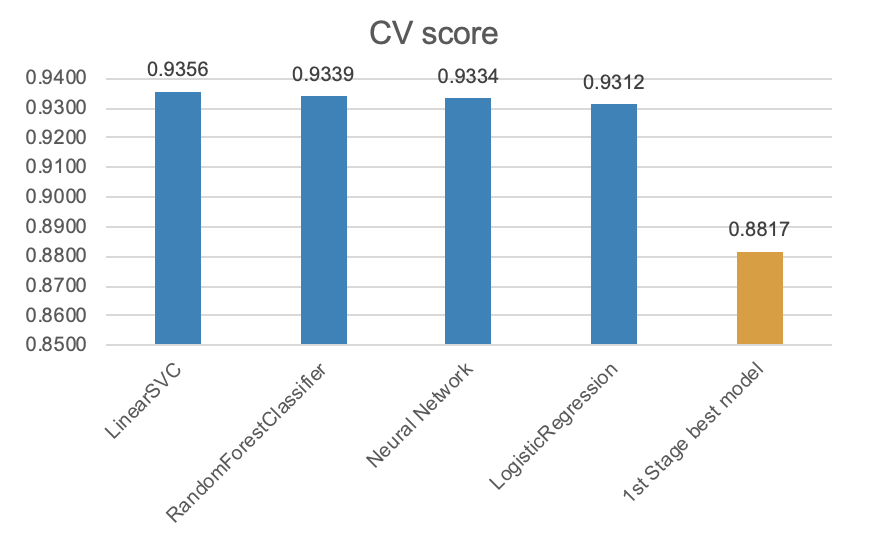
\includegraphics[scale=0.8]{./Figure/2ndstage.png}
        \caption{2nd Stage models CV accuracy score}
        \label{fig:2ndstage}
      \end{figure}

From these results of 2nd stage we could see that our all models score are better than the best score from 1st stage. Moreover, comparing to the best model at this stage we have a difference of about 5.39\verb+%+ from the 1st stage best model. This fact could prove that our Stacking method is useful and very powerful method to improve the performance of malware detection systems or models.